Raviolimaskinen som kommer utvecklas för detta projekt består av några viktiga delar. Detta består av en pump som ska hälla raviolis ifyllnings material på degen. För detta måste man ha kunskap om hur en pump fungerar, vilkar delar en pump har och hur man ska designa det för att det ska passa just detta projekt.\medskip

En annan del är formen på degen. På figuren ~\ref{degfrom} visas en degform som används för att knyta degen manuellt genom att trycka på formens sidor. För detta projekt har funderats på att utveckla en degform som kan styras med en eller två motorer. En viktig uppgift är att man kan  överföra motorers energi på så sätt att formen får tillräcklig kraft för att knyta degen. Det kommer finnas kugghjul för energiöverföringen från motor till degformen. Kunskapen inom olika typer av kugghjul och hur ett kugghjul fungerar ska utvecklas.\medskip

\begin{figure}[h]
	\begin{center}
		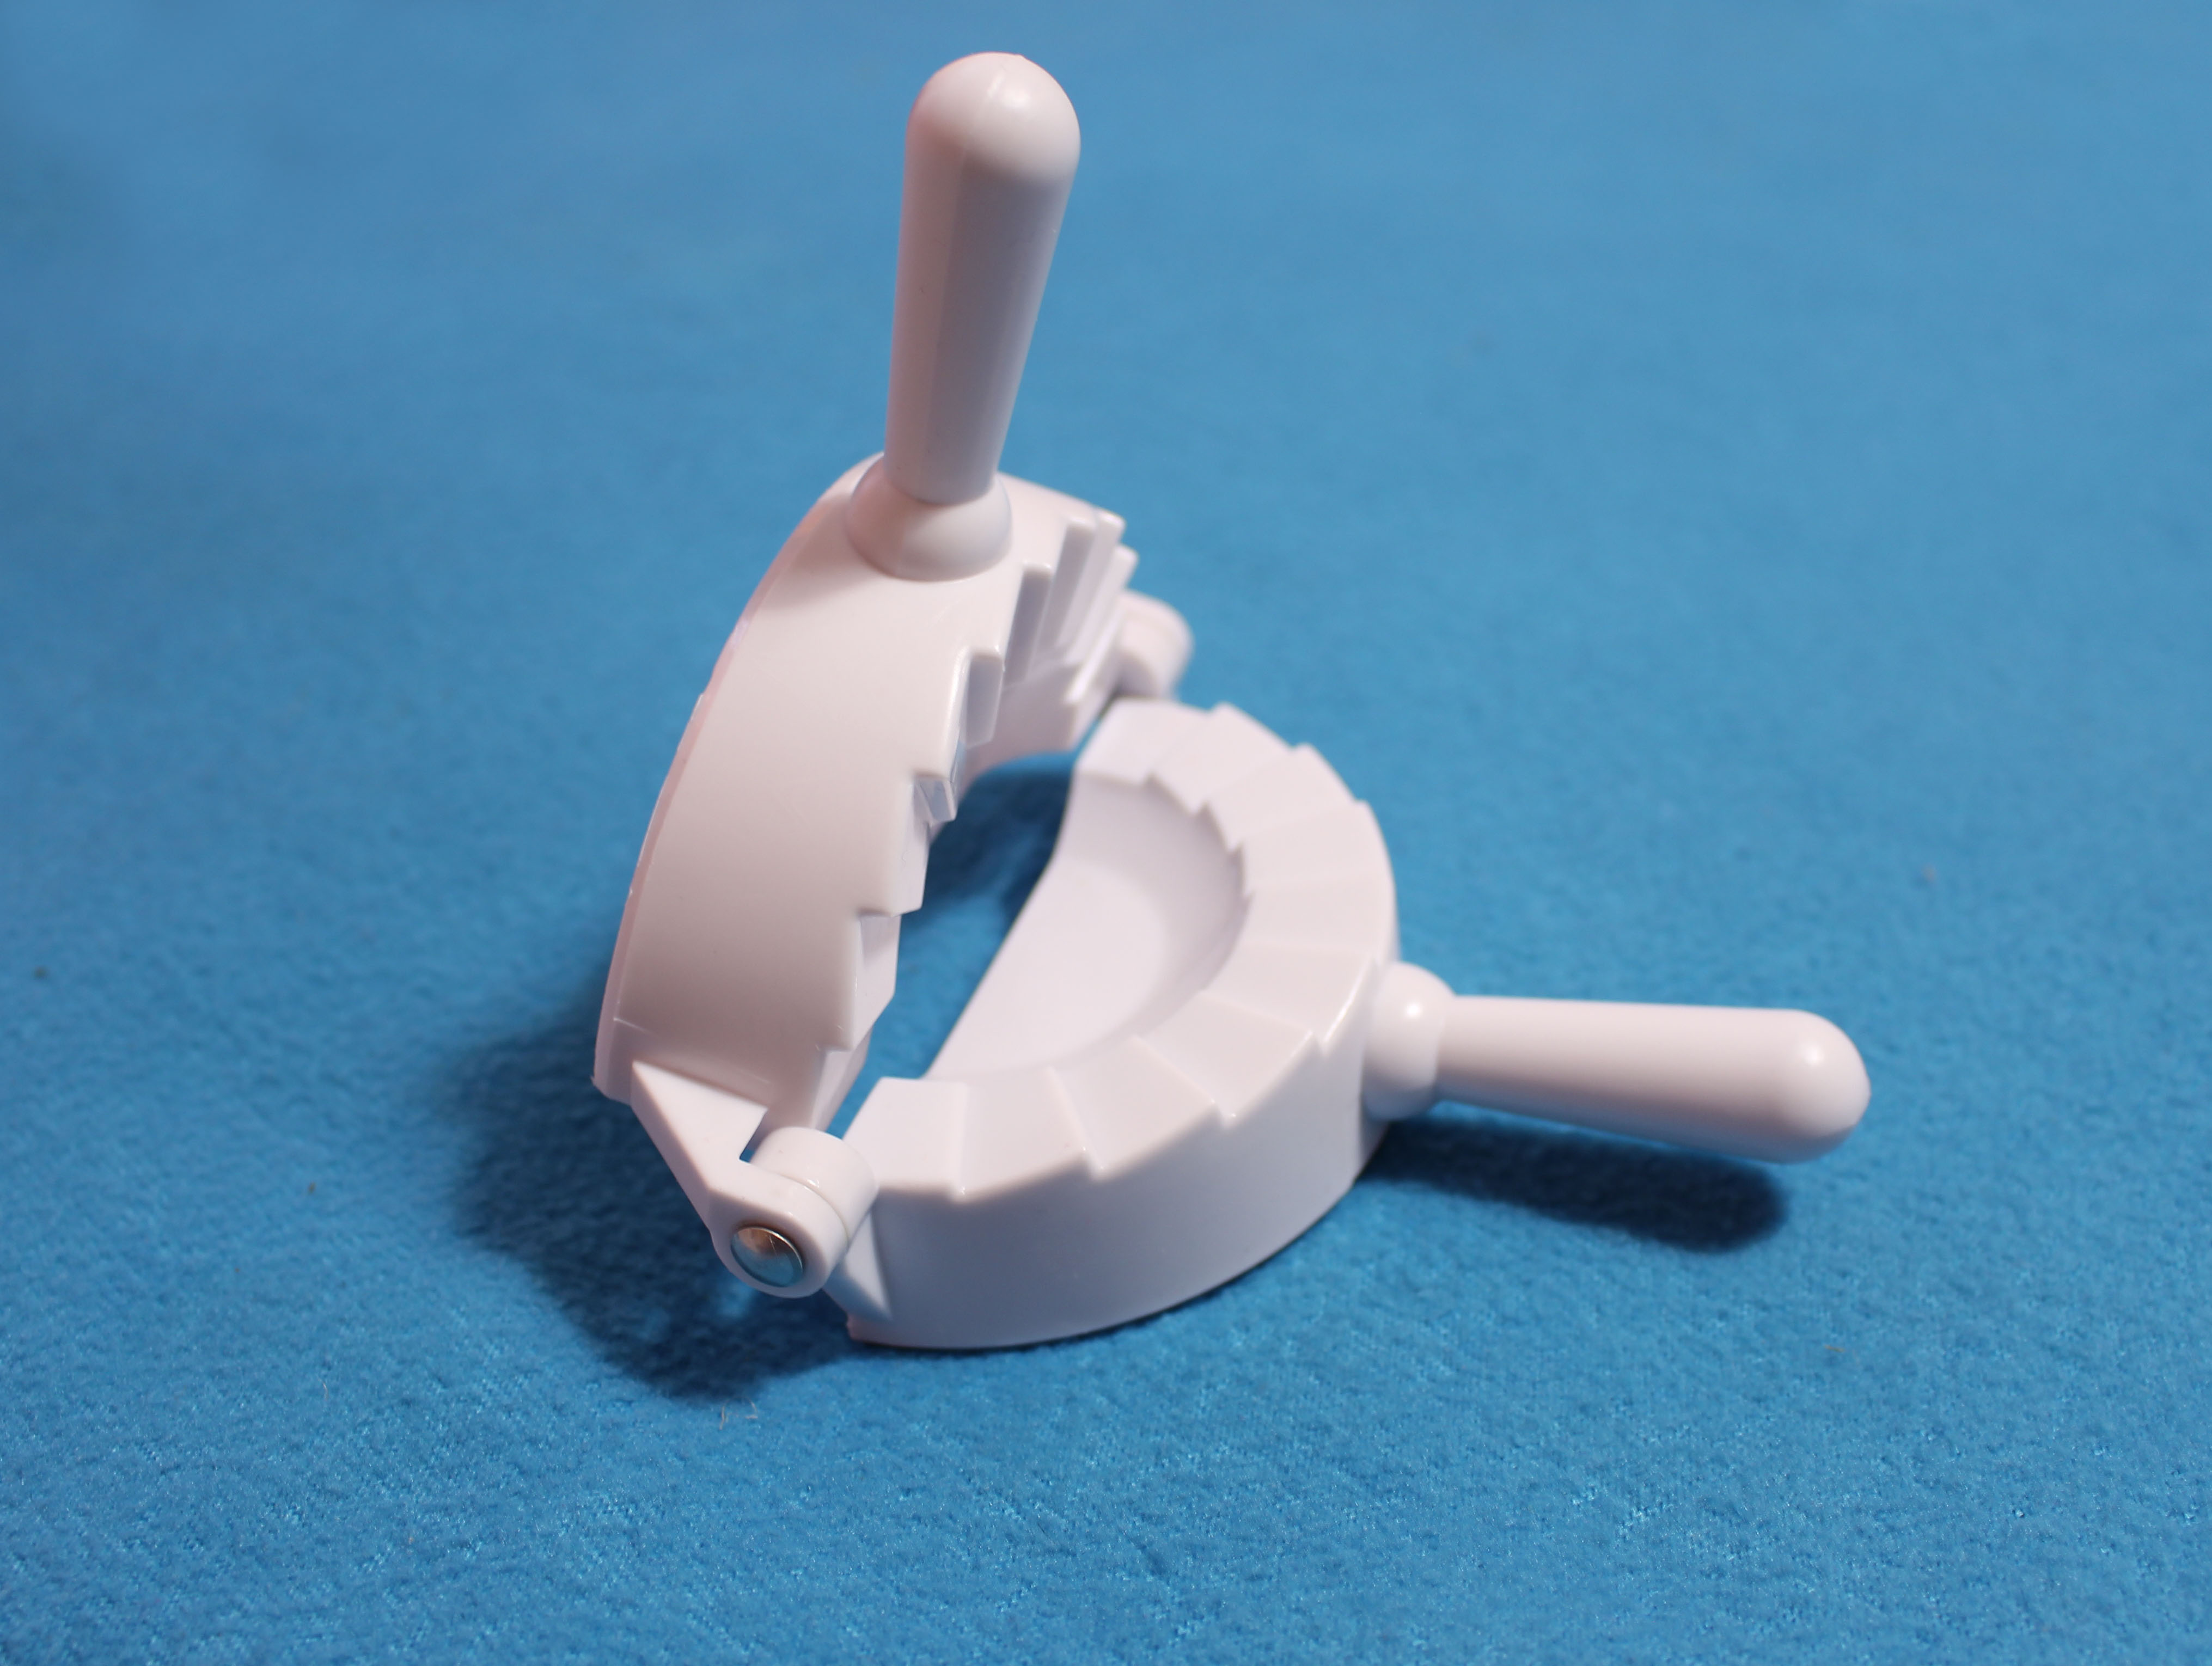
\includegraphics[scale=0.08] {images/degform.jpg}
		\caption{Degform för manuell ifyllning}
		\label{degfrom}	
	\end{center}
\end{figure}\medskip

För att alla Raviolimaskinens delar ska fungera ihop och varje del gör sin uppgift i rätt tid, måste det finnas en enhet för att kontrollera dem. Kontrol av alla delar görs m.h.a. en mikrokontroller som bestämmer vad som ska hända i varje tidspunkt. Olika typer av mikrokontroller måste analyseras för att hitta den som passar bäst till projektet.

Det kommer möjligen finnas reglator som kommer reglera strömmen som ska driva motorer. Man läser om olika regleringsmetoder under programmet, men kunskapen att implementera en analog regulator måste utvecklas.




